\documentclass{beamer}

\mode<presentation>{%
  \usetheme[block=fill,progressbar=frametitle]{metropolis}
  \setsansfont[BoldFont={Fira Sans SemiBold}]{Fira Sans Book}
}

\usepackage{appendixnumberbeamer}
\usepackage[font=tiny]{caption}
\usepackage{graphicx}
% \usepackage{natbib}
\usepackage{bibentry}
\usepackage{booktabs}

\title{Network Measures of Gene Flow}
\author{Ansel George}
\date{\today}

\begin{document}

\begin{frame}
\titlepage%
\end{frame}

\section{Introduction}

\begin{frame}{Gene Flow}
  \begin{block}{Problem}
    How does one infer potentially complex evolutionary phenomena?
  \end{block}
\end{frame}

\begin{frame}{Gene Flow}
  \begin{block}{Problem}
    How does one infer potentially complex evolutionary phenomena?
  \end{block}
  Depends on:
  \begin{itemize}
    \item Genetic variation within populations
    \item Migration rates
    \item Selection
    \item Patterns in mating and reproduction (e.g.\ speciation)
    \item \dots
  \end{itemize}
\end{frame}

\begin{frame}{Gene Flow}
  \begin{block}{Problem}
    How does one infer potentially complex evolutionary phenomena?
  \end{block}
  \begin{itemize}
    \item All of these contributing factors can vary in intensity temporally
      and spatially.
    \item Dynamics can be \textit{extremely} complex.
    \item Many methods and simplifying models exist.
  \end{itemize}
\end{frame}

\begin{frame}{Goal}
  \begin{block}{Question 1}
    Can network/graphical methods be used to study gene flow?
  \end{block}

  \vspace{2em}

  \begin{block}{Question 2}
    How effective are those methods compared to others?
  \end{block}
\end{frame}

\section{The Data}

\begin{frame}{SNP Arrays}
  \begin{itemize}
    \item Individuals vary in genotype across loci.
    \item Point variations in DNA sequence are single nucleotide polymorphisms
      (SNPs).
    \item SNPs across many samples are agglomerated to estimate population
      parameters.
    \item \textit{Important:} These methods usually assume alleles are at or
      near Hardy-Weinberg equilibrium.
  \end{itemize}
\end{frame}

% \begin{frame}{Genetic Distance Estimators}
% \end{frame}

\section{Model-based Methods}

\begin{frame}{structure/ADMIXTURE}
  \begin{itemize}
    \item Use a Bayesian model for inferring population
      structure~\cite{pritchard_inference_2000,falush_inference_nodate,alexander_fast_2009}.
      \begin{align*}
        P(Z,\Theta|X) &\approx P(Z)P(\Theta)P(X|Z,\Theta)
      \end{align*}
    \item Clusters individuals based on likelihood of coming from
      subpopulation.
    \item Assumes independence of loci.
    \item Uses Markov Chain Monte Carlo and Gibbs sampling to estimate
      parameters for subpopulations from SNP data.
    \item Can infer admixture of individuals.
  \end{itemize}
\end{frame}

% \begin{frame}{Trees}
%   Hi there.~\cite{corander_bayesian_nodate}
% \end{frame}

\section{Dimensionality Reduction Methods}

\begin{frame}{Principal Components Analysis (PCA)}
  \begin{itemize}
    \item Computed by eigendecomposition of the genotype covariance matrix.
      \begin{align*}
        \textbf{M} &= \frac{1}{n} \textbf{X}^T\textbf{X} = \textbf{V} \textbf{$\Lambda$} \textbf{V}^T
      \end{align*}
    \item Projects samples into feature (genotype)-space.
    \item Loadings of 1st component correspond to ratio of inter-group to total
      variance ($F_{st}$)~\cite{mcvean_genealogical_2009}.
  \end{itemize}
\end{frame}

\begin{frame}{Principal Components Analysis (II)}
  \begin{columns}
    \begin{column}{0.48\textwidth}
      \begin{itemize}
        \item Identify admixed individuals by projecting their genotypes onto
          the principal component vectors constructed from reference
          populations.
        \item Detects gene flow with simple linear transformation of data!
      \end{itemize}
    \end{column}
    \begin{column}{0.48\textwidth}
      \begin{figure}
        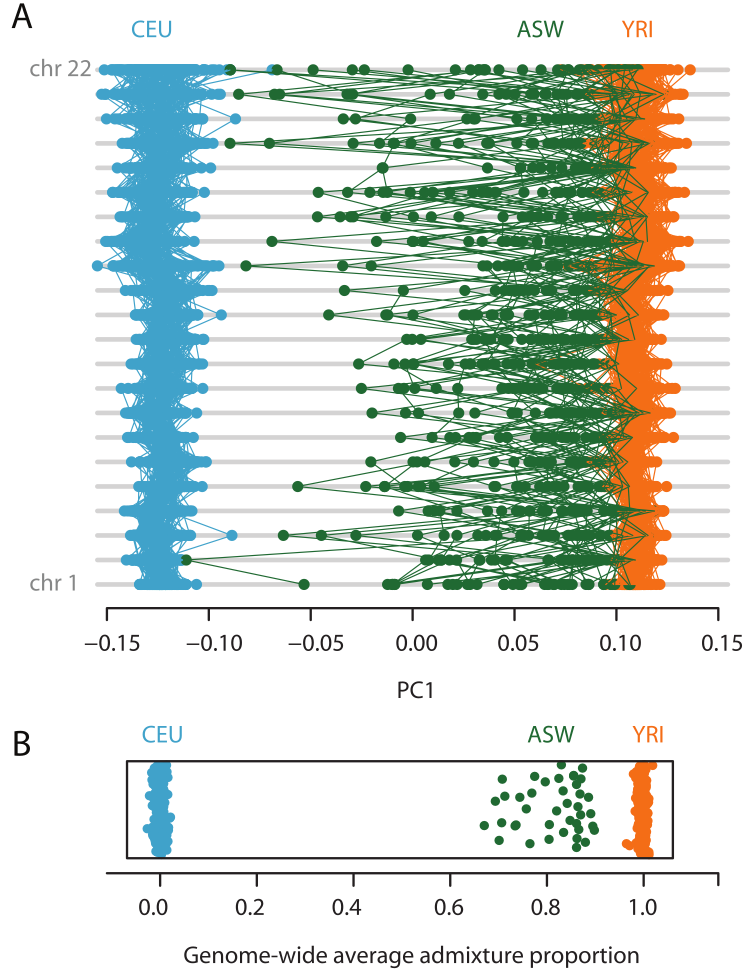
\includegraphics[width=\linewidth,keepaspectratio]{../Figures/fig3.png}
        \caption{Position of admixed individuals (green) along principal
          component axes defined by European (blue) and Yoruban (orange)
          populations~\cite{mcvean_genealogical_2009}.}
      \end{figure}
    \end{column}
  \end{columns}
\end{frame}

\begin{frame}{Principal Components Analysis (III)}
  \textit{Drawback:} PCA separation from admixture is lost over
  time~\cite{mcvean_genealogical_2009}.
  \begin{figure}
    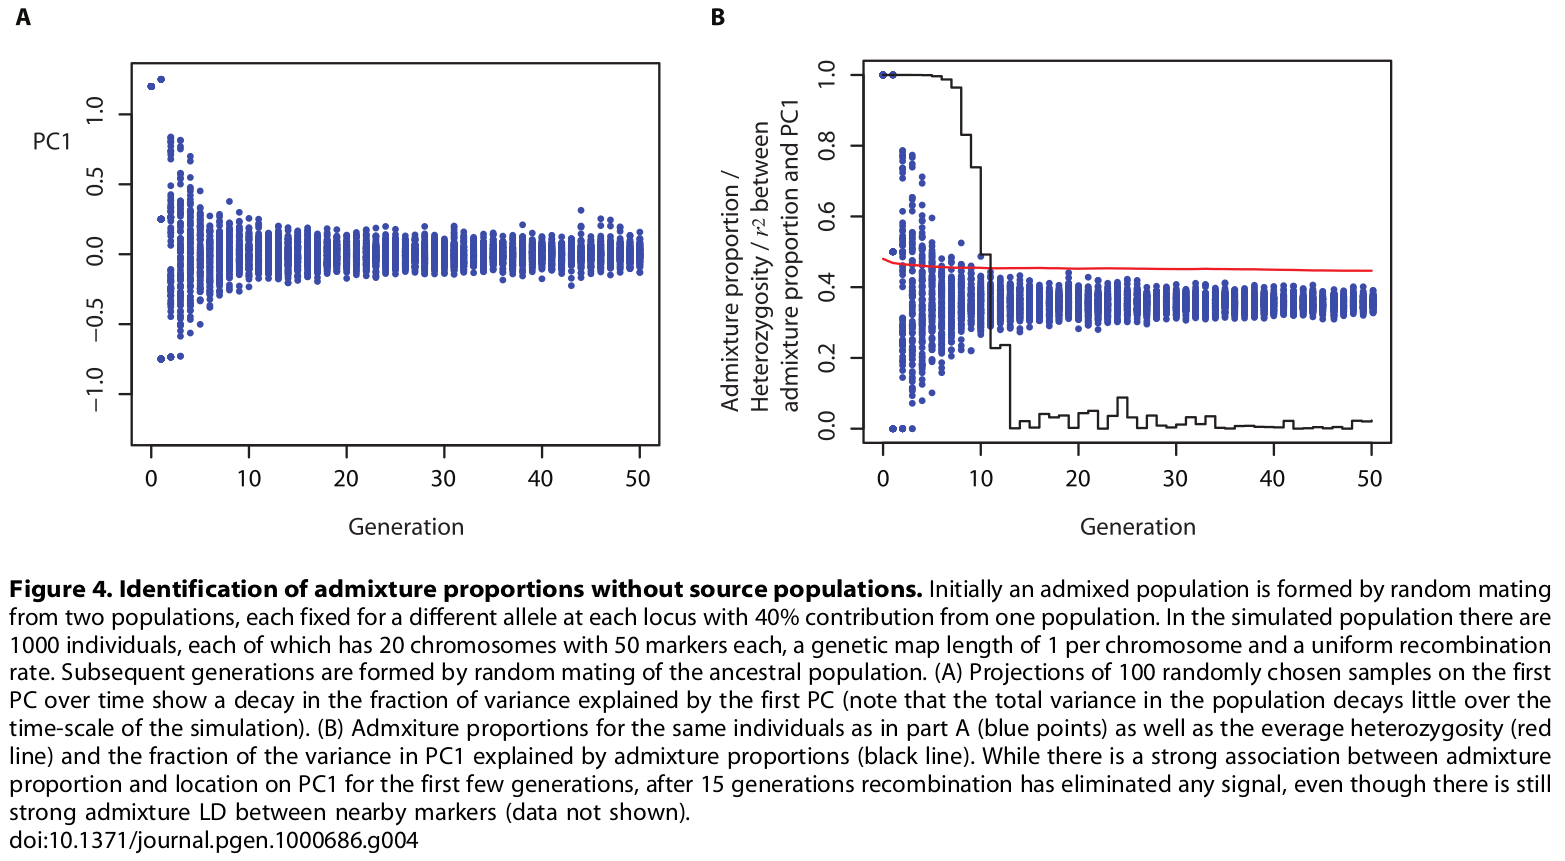
\includegraphics[width=\linewidth,keepaspectratio]{../Figures/fig1.png}
    \caption{See G. McVean. A genealogical interpretation of principal
    components analysis.}
  \end{figure}
\end{frame}

\begin{frame}{Principal Components Analysis (IV)}
  \begin{itemize}
    \item \textit{Very} vulnerable to outliers.
      \begin{itemize}
        \item SNP calls for rare variants are not possible for small samples
          sizes or low read coverage.
      \end{itemize}
    \item \textit{Very} susceptible to non-uniform sampling.
  \end{itemize}
\end{frame}

\begin{frame}{Principal Components Analysis (V)}
  \begin{figure}
    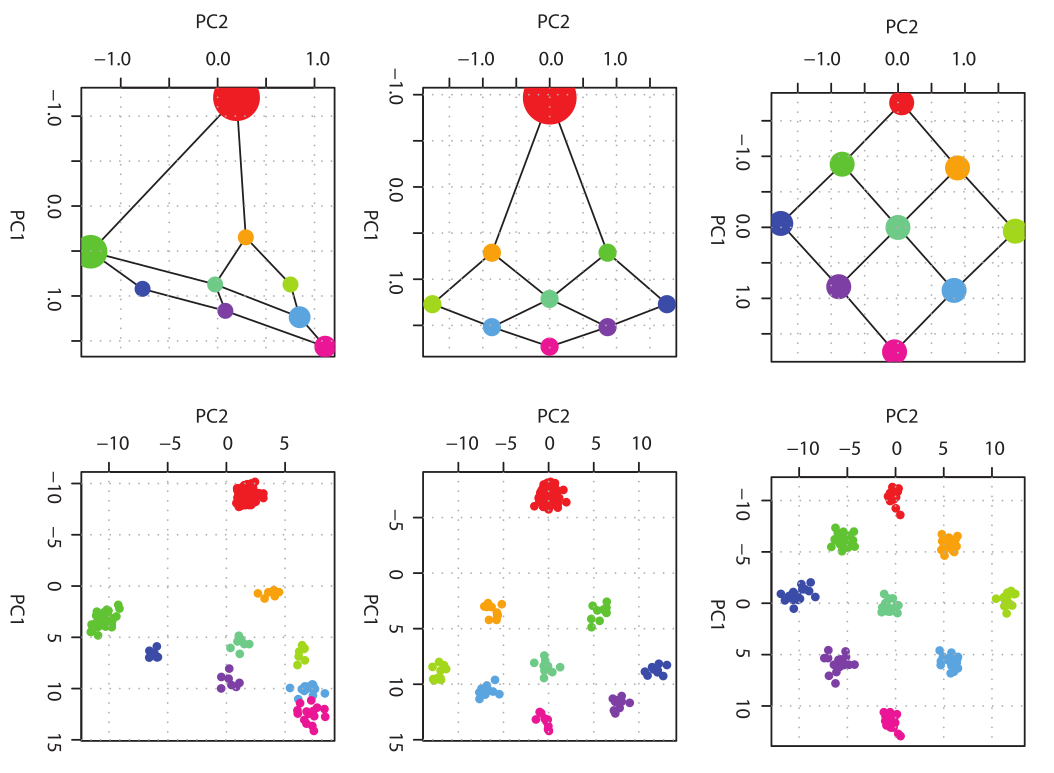
\includegraphics[width=.9\linewidth,keepaspectratio]{../Figures/fig2.png}
    \caption{Principal component distances get skewed by sample size (area of
      dot) for each deme~\cite{mcvean_genealogical_2009}.}
  \end{figure}
\end{frame}

\section{Network-based Methods}

\begin{frame}{Population Graphs}
  Computes graph structure based on genetic similarity of
  demes~\cite{dyer_population_2004}.
  \begin{enumerate}
    \item Group individuals by sample.
    \item Compute genotype centroids corresponding to each sample.
    \item Generate distance matrix $D$ for each pair of centroids.
    \item Compute covariance matrix $\Sigma$ for $D$.
    \item Compute precision matrix ($\Omega = \Sigma^{-1}$) for covariance
      structure.
  \end{enumerate}
\end{frame}

\begin{frame}{Population Graphs (II)}
  \begin{enumerate}
    \setcounter{enumi}{5}
    \item Prune graph by removing edges with 0 entries in $\Omega$. 
      \begin{itemize}
        \item $\Omega_{ij} = 0$ means $i\rightarrow j$ is conditionally independent.
        \begin{equation*}
          P(A,B|C) = P(A|C) P(B|C)
        \end{equation*}
        \item Use Edge Exclusion Deviance (EED) to remove edges not
          significantly different from 0.
      \end{itemize}
        \begin{equation*}
          EED = -{n} \log{(1-r_{ij}^2)}
        \end{equation*}
    \item Compute model deviance to check that resulting graph maintains
      covariance structure of original data.
    \begin{equation*}
      D = {n} \log\frac{|\Sigma|}{|S|}
    \end{equation*}
  \end{enumerate}
\end{frame}

\begin{frame}{Population Graphs (III)}
  The resulting graph is amenable to the usual battery of network measures.
  \begin{figure}
    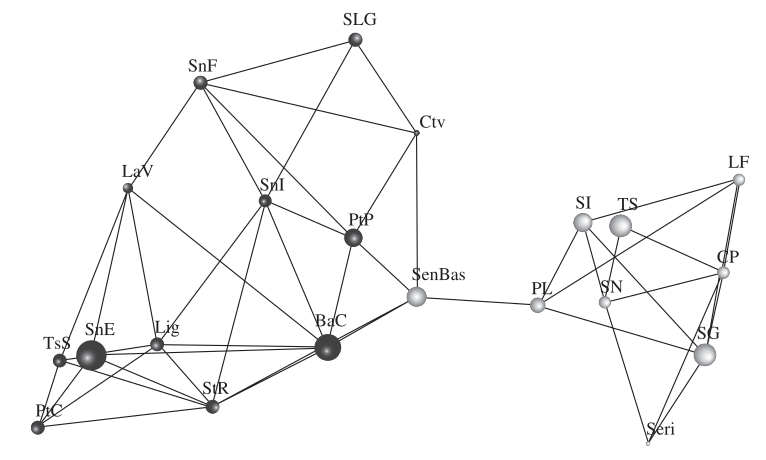
\includegraphics[width=.9\linewidth,keepaspectratio]{../Figures/fig4.png}
    \caption{Population graph for \textit{L. schottii}
    dataset.}
  \end{figure}
\end{frame}

\begin{frame}{Population Graphs (IV)}
  The Population Graph method has found populations with small-world network
  structures~\cite{garroway_applications_2008}.
  \begin{itemize}
    \item Degree and eigenvector centrality $\rightarrow$ proportion of
      migrants (empirical; related to habitat suitability).
    \item Shortest path length between nodes $\rightarrow$ $F_{st}$.
    \item Degree distribution $\rightarrow$ network generative model.
    \item Modularity $\rightarrow$ whether subpopulations exist.
  \end{itemize}
\end{frame}

\begin{frame}{Population Graphs (V)}
  Drawbacks:
  \begin{enumerate}
    \item Computing precision matrix is numerically unstable.
    \item Connectivity depends on arbitrary distance thresholds.
    \item Nodes with high betweenness in simplified graph could be an
      artefact of simplification process.
    \item Permutations require sequential removal of nodes and recomputing
      graphs. (Expensive for large datasets.)
  \end{enumerate}
\end{frame}

\begin{frame}{NetView\cite{neuditschko_netview:_2012}}
  \begin{itemize}
    \item Computes genetic distances among individuals using allele sharing
      distance (ASD)~\cite{gao_using_2009,purcell_plink:_2007}.
      \begin{align*}
        D &= \frac{1}{L} \sum_{i=1}^L d_i\textrm{, where} \\
          &d_i = 0\textrm{ if individuals have both alleles in common, } \\
          &d_i = 1\textrm{ if individuals have 1 allele in common, and } \\
          &d_i = 2\textrm{ if individuals have no alleles in common}
      \end{align*}
    \item Nodes representing individuals are constructed into a graph by
      nearest-neighbor joining.
    \item Nodes are clustered with SPC\@ where edge widths correspond to
      strength of genetic similarity.
  \end{itemize}
\end{frame}

\begin{frame}{NetView (II)}
  \begin{figure}
    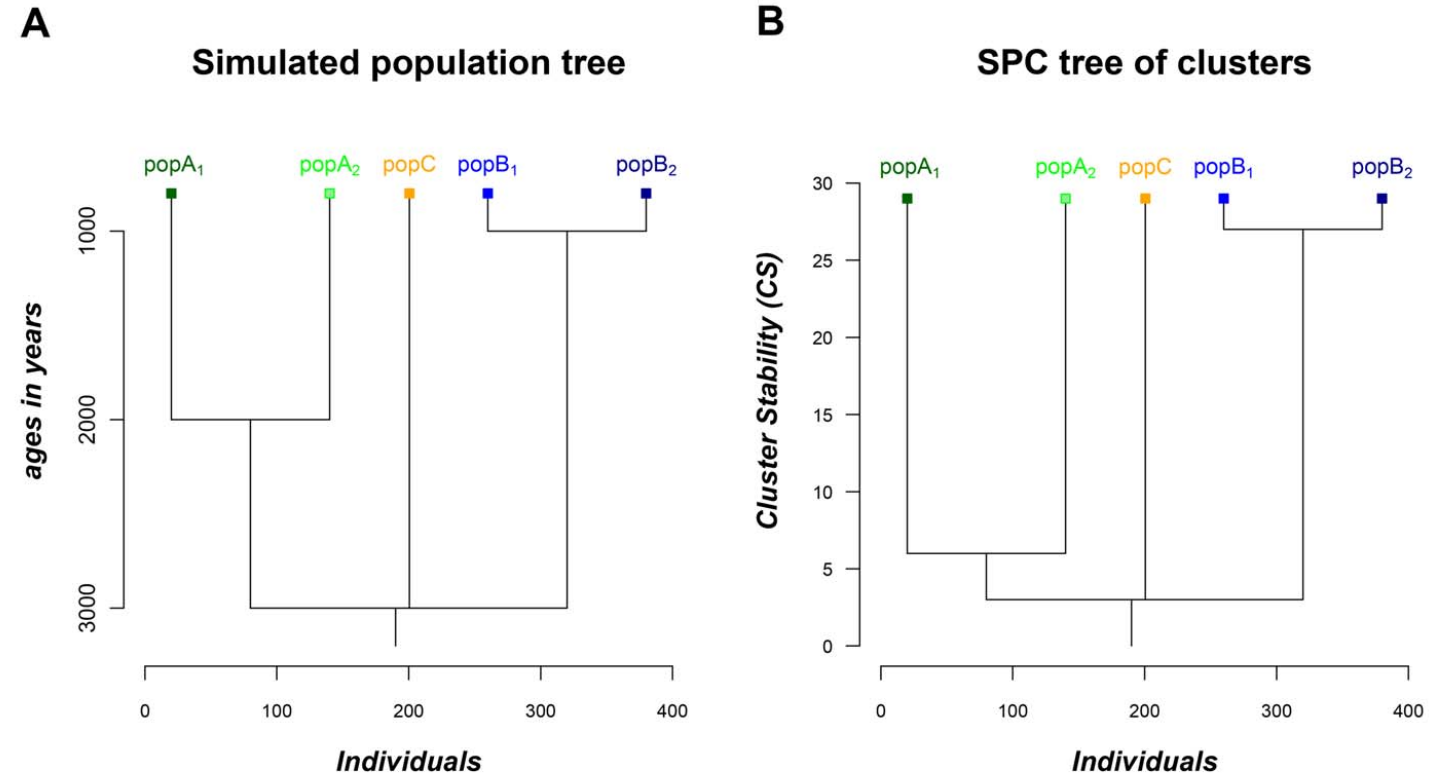
\includegraphics[width=1\linewidth,keepaspectratio]{../Figures/fig6ab.png}
    \caption{Simulated population structure. Strong SPC cluster stability
    corresponds to strong interrelatedness within the cluster.}
  \end{figure}
\end{frame}

\begin{frame}{NetView (III)}
  The cluster forms a network structure amenable to network analysis (e.g.\
  within-cluster degree distributions, modularity, etc.)
  \begin{figure}
    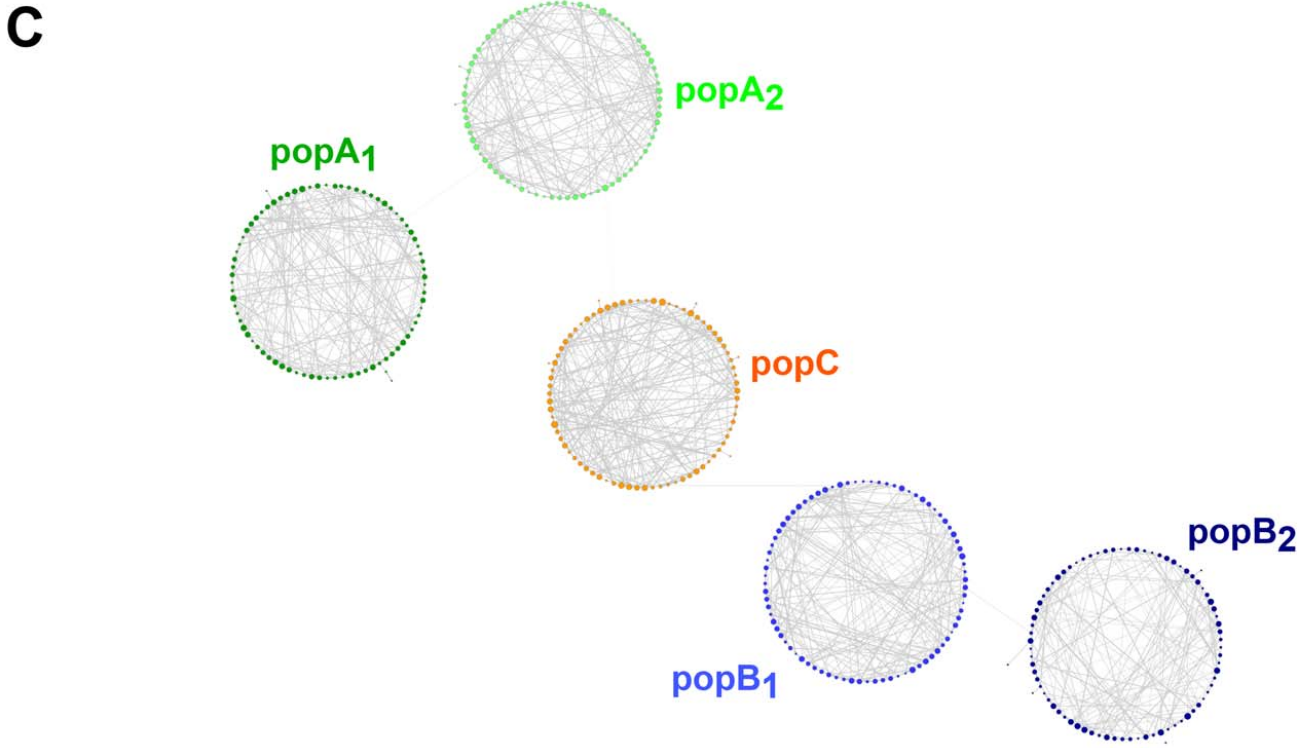
\includegraphics[width=1\linewidth,keepaspectratio]{../Figures/fig6c.png}
    \caption{SPC clusters for the population graph. All individuals were
    classified correctly.}
  \end{figure}
\end{frame}

\section{Conclusions}

\begin{frame}{Summary}
  \begin{block}{Question 1}
    Can network/graphical methods be used to study gene flow?
  \end{block}

  \textbf{Yes!}
  \vspace{1em}

  \begin{block}{Question 2}
    How effective are network methods compared to others?
  \end{block}

  \textit{Maybe better, maybe not\ldots}
\end{frame}

\begin{frame}{Future Work}
  \begin{itemize}
    \item Evaluate network methods and compare for:
      \begin{itemize}
        \item Computational performance
        \item Vulnerability to outliers and missing variants
        \item Ability to resolve different evolutionary phenomena
        \item How one-to-one is the relationship between data and results
      \end{itemize}
    \item Can they be extended to temporal samples? (e.g.~ancient DNA)
  \end{itemize}
\end{frame}


\begin{frame}[allowframebreaks]{References}
  % \bibliographystyle{plainnat}
  % \bibliographystyle{abbrvnat}
  \bibliography{publications}
  \bibliographystyle{abbrv}
\end{frame}

\begin{frame}[label=end, standout]
\end{frame}

% \appendix
% 
% \begin{frame}
% \end{frame}

\end{document}
